\documentclass{report}

\usepackage[T2A]{fontenc}
\usepackage[utf8]{luainputenc}
\usepackage[english, russian]{babel}
\usepackage[pdftex]{hyperref}
\usepackage[14pt]{extsizes}
\usepackage{color}
\usepackage{geometry}
\usepackage{enumitem}
\usepackage{multirow}
\usepackage{graphicx}
\usepackage{indentfirst}
\usepackage{amsmath}
\usepackage{listings}
\usepackage{xcolor}
\usepackage{multicol}

%New colors defined below
\definecolor{codegreen}{rgb}{0,0.6,0}
\definecolor{codegray}{rgb}{0.5,0.5,0.5}
\definecolor{codepurple}{rgb}{0.58,0,0.82}
\definecolor{backcolour}{rgb}{0.95,0.95,0.92}

%Code listing style named "mystyle"
\lstdefinestyle{mystyle}{
  backgroundcolor=\color{backcolour},   commentstyle=\color{codegreen},
  keywordstyle=\color{magenta},
  numberstyle=\tiny\color{codegray},
  stringstyle=\color{codepurple},
  basicstyle=\ttfamily\footnotesize,
  breakatwhitespace=false,         
  breaklines=true,                 
  captionpos=b,                    
  keepspaces=true,                 
  numbers=left,                    
  numbersep=5pt,                  
  showspaces=false,                
  showstringspaces=false,
  showtabs=false,                  
  tabsize=2
}

%"mystyle" code listing set
\lstset{style=mystyle}

\geometry{a4paper,top=1cm,bottom=2cm,left=1cm,right=1cm}
\setlength{\parskip}{0.5cm}
\setlist{nolistsep, itemsep=0.3cm,parsep=0pt}

\begin{document}

\newpage
\par \textbf{Задание №1}

\par 1)
\begin{align*}
& a \in \mathbf{R}^N, x \in \mathbf{R}^N \\
& a^T x: \mathbf{R}^N \rightarrow \mathbf{R}^1 \Rightarrow \frac{\partial a^T x}{\partial x} = \nabla_x (a^T x) \\
& a^T x = \begin{pmatrix} a_1 & a_2 & \cdots & a_N \end{pmatrix} \begin{pmatrix} x_1 \\ x_2 \\ \cdots \\ x_N \end{pmatrix} = \sum_{i=1}^{N} a_i x_i \\
& \frac{\partial a^T x}{\partial x} = \frac{\partial \left( \sum_{i=1}^{N} a_i x_i \right)}{\partial x} = \begin{pmatrix} \frac{\partial a_1 x_1}{\partial x_1} \\ \frac{\partial a_2 x_2}{\partial x_2} \\ \cdots \\ \frac{\partial a_N x_N}{\partial x_N} \end{pmatrix} = a
\end{align*}

\par 2)
\begin{align*}
& Ax: \mathbf{R}^{m \times n} \rightarrow \mathbf{R}^m \\
& \frac{\partial Ax}{\partial x} = \begin{pmatrix}
\frac{\partial \left( \sum_{i=1}^{N} a_{1i} x_i \right)}{\partial x_1} &&
\frac{\partial \left( \sum_{i=1}^{N} a_{1i} x_i \right)}{\partial x_2} &&
\cdots &&
\frac{\partial \left( \sum_{i=1}^{N} a_{1i} x_i \right)}{\partial x_n} \\
\cdots && \cdots && \cdots && \cdots \\
\frac{\partial \left( \sum_{i=1}^{N} a_{mi} x_i \right)}{\partial x_1} &&
\frac{\partial \left( \sum_{i=1}^{N} a_{mi} x_i \right)}{\partial x_2} &&
\cdots &&
\frac{\partial \left( \sum_{i=1}^{N} a_{mi} x_i \right)}{\partial x_n}
\end{pmatrix} = \\
& = \begin{pmatrix}
a_{11}  && a_{12} && \cdots && a_{1n} \\
\cdots && \cdots && \cdots && \cdots \\
a_{m1}  && a_{m2} && \cdots && a_{m n}
\end{pmatrix} = A
\end{align*}

\par 3)
\begin{align*}
& A \in \mathbf{R}^{N \times N} \\
& \frac{\partial ( x^T Ax )}{\partial x} = (A + A^T) x \\
& x^T Ax = \sum_{i=1}^{N} x_i \sum_{j=1}^{N} a_{i j} x_j \\
& \frac{\sum_{i=1}^{N} x_i \sum_{j=1}^{N} a_{i j} x_j}{\partial x_k} =
\frac{\partial \left(
    a_{k k} x_k^2 +
    \sum_{i=1, i \neq k}^{N} x_i \sum_{j=1}^{N} a_{i j} x_j +
    \sum_{i=1}^{N} x_i \sum_{j=1, j \neq k}^{N} a_{i j} x_j   
\right)}{\partial x_k} = \\
& = 2 a_{k k} x_k + \sum_{i=1, i \neq k}^{N} a_{i k} x_k + \sum_{j = 1, j \neq k}^{N} a_{k j} x_k
= \sum_{i=1}^{N} a_{i k} x_k + \sum_{j=1}^{N} a_{k j} x_k = \sum_{i = 1}^{N} x_k (a_{i k} + a_{k i} ) \\
& \frac{\partial ( x^T Ax )}{\partial x} = \begin{pmatrix}
    \frac{\partial \left( \sum_{i=1}^{N} x_i \sum_{j=1}^{N} a_{i j} x_i \right)}{\partial x_1} \\
    \cdots \\
    \frac{\partial \left( \sum_{i=1}^{N} x_i \sum_{j=1}^{N} a_{i j} x_i \right)}{\partial x_N}
\end{pmatrix} = \begin{pmatrix}
    \sum_{i=1}^{N} x_1 (a_{i1} + a_{1i}) \\
    \cdots \\
    \sum_{i=1}^{N} x_N (a_{i N} + a_{N i})
\end{pmatrix} = \\
& = \begin{pmatrix}
    a_{11}+a_{11} & a_{21}+a_{12} & \cdots & a_{n1}+a_{1n} \\
    \cdots & \cdots & \cdots & \cdots \\
    a_{1n}+a_{n1} & \cdots & \cdots & a_{n n}+a_{n n}
\end{pmatrix} \begin{pmatrix} x_1 \\ \cdots \\ x_N \end{pmatrix} = (A + A^T) x \\
& \text{В частности, если } A = A^T, \text{ то } \frac{\partial ( x^T Ax )}{\partial x} = 2Ax
\end{align*}

\par 4)
\begin{align*}
& \|x\|^2 = ( \sqrt{x^T x} )^2 = x^T x = \sum_{i=1}^{N} x_i^2;
\frac{\partial \|x\|^2}{\partial x} = \begin{pmatrix}
    \frac{\partial \left( \sum_{i=1}^{N} x_i^2 \right)}{\partial x_1} \\
    \cdots \\
    \frac{\partial \left( \sum_{i=1}^{N} x_i^2 \right)}{\partial x_N}
\end{pmatrix} = 2x
\end{align*}

\par 5)
\begin{align*}
& \frac{\partial g(x)}{\partial x} = \begin{pmatrix}
    \frac{\partial g(x_1)}{\partial x_1} & \frac{\partial g(x_2)}{\partial x_1} & \cdots & \frac{\partial g(x_N)}{\partial x_1} \\
    \cdots & \cdots & \cdots & \cdots \\
    \frac{\partial g(x_1)}{\partial x_N} & \cdots & \cdots & \frac{\partial g(x_N)}{\partial x_N}
\end{pmatrix} \overset{(*)}{=} \begin{pmatrix}
    g \prime (x_1) & 0 & \cdots & 0 \\
    0 & g \prime (x_2) & \cdots & 0 \\
    \cdots & \cdots & \cdots & \cdots \\
    0 & 0 & \cdots & g \prime (x_N)
\end{pmatrix} = \\
& = \text{diag}(g \prime (x)) \\ \\
& (*) \frac{\partial g(x_i)}{\partial x_j} = \begin{cases}
    g \prime (x_i), i \neq j \\
    0, i \neq j
\end{cases}
\end{align*}

\par 6)
\begin{align*}
& x \in \mathbf{R}^n; h: \mathbf{R}^n \rightarrow \mathbf{R}^m; g: \mathbf{R}^m \rightarrow \mathbf{R}^p \\
& \frac{\partial g(h(x))}{\partial x} = \begin{pmatrix}
    \frac{\partial g_1 (h(x))}{\partial x_1} & \cdots & \frac{\partial g_1 (h(x))}{\partial x_n} \\
    \cdots & \cdots & \cdots \\
    \frac{\partial g_p (h(x))}{\partial x_1} & \cdots & \frac{\partial g_p (h(x))}{\partial x_n} \\
\end{pmatrix} \overset{(*)}{=} \\
& \overset{(*)}{=} \begin{pmatrix}
    \sum_{i=1}^{n} \frac{\partial g_1 (h(x))}{\partial h_i} \cdots \frac{\partial h_i (x)}{\partial x_1} &
    \cdots &
    \sum_{i=1}^{n} \frac{\partial g_1 (h(x))}{\partial h_1} \cdots \frac{\partial h_i (x)}{\partial x_n} \\
    \cdots & \cdots & \cdots \\
    \sum_{i=1}^{n} \frac{\partial g_p (h(x))}{\partial h_i} \cdots \frac{\partial h_i (x)}{\partial x_1} &
    \cdots &
    \sum_{i=1}^{n} \frac{\partial g_p (h(x))}{\partial h_1} \cdots \frac{\partial h_i (x)}{\partial x_n}
\end{pmatrix} = \\
& = \begin{pmatrix}
    \frac{\partial g_1 (h(x))}{\partial h_1} & \frac{\partial g_1 (h(x))}{\partial h_2} & \cdots & \frac{\partial g_1 (h(x))}{\partial h_m} \\
    \cdots & \cdots & \cdots & \cdots \\
    \frac{\partial g_p (h(x))}{\partial h_1} & \frac{\partial g_p (h(x))}{\partial h_2} & \cdots & \frac{\partial g_p (h(x))}{\partial h_m}
\end{pmatrix} \cdot \begin{pmatrix}
    \frac{\partial h_1 (x)}{\partial x_1} & \cdots & \frac{\partial h_1 (x)}{\partial x_n} \\
    \cdots & \cdots & \cdots \\
    \frac{\partial h_m (x)}{\partial x_1} & \cdots & \frac{\partial h_m (x)}{\partial x_n}
\end{pmatrix} = \frac{\partial g(h(x))}{\partial h} \cdot \frac{\partial h(x)}{\partial x} \\ \\
& (*) \frac{\partial g_k (h(x)}{\partial x_i} =
    \frac{\partial g_k (h(x))}{\partial h_1} \cdot \frac{\partial h_1 (x)}{\partial x_i} +
    \frac{\partial g_k (h(x))}{\partial h_2} \cdot \frac{\partial h_2 (x)}{\partial x_i} +
    \cdots +
    \frac{\partial g_k (h(x))}{\partial h_m} \cdot \frac{\partial h_m (x)}{\partial x_i}
\end{align*}

\newpage
\par \textbf{Задание №2}

\par Пусть $ g(\beta) = \|X \beta - y\|^2$. Покажем, что $\beta^* = \arg \min \|X\beta - y\|$ является решением системы линейных уравнений $X^T X\beta = X^T y$.

\par Найдем градиент $\frac{\partial g(\beta)}{\partial \beta}$.
\begin{align*}
& \frac{\partial g(\beta)}{\partial \beta} = \frac{\partial}{\partial \beta} \left( \|X\beta - y\|^2 \right) =
\frac{\partial}{\partial \beta} \left( (X\beta - y)^T (X\beta - y) \right) = \\
& = \frac{\partial}{\partial \beta} (\beta^T X^T X \beta - \beta^T X^T y - y^T X \beta + y^T y) \overset{(*)}{=} \\
& = \frac{\partial}{\partial \beta} (\beta^T X^T X \beta - 2 \beta^T X^T y + y^T y) \overset{(**)}{=} 2 X^T X \beta - 2 X^T y \\ \\
& (*) y^T X \beta = ((y^T X) \beta)^{T T} = (\beta^T (y^T X)^T)^T = (\beta^T X^T y)^T = \beta^T X^T y \\
& (**) \begin{cases}
    \frac{\partial}{\partial \beta} (\beta^T X^T X \beta) \overset{A = X^T X}{=} \frac{\partial}{\partial \beta} (\beta^T A \beta) = 2A \beta = 2 X^T X \beta \\
    \frac{\partial}{\partial \beta} (2 \beta^T X^T y) = 2X^T y \\
    \frac{\partial}{\partial \beta} (y^T y) = 0
\end{cases}
\end{align*}

\par Найдем точку, подозрительную на экстремум:
\begin{align*}
& \frac{\partial g(\beta)}{\partial \beta} = 0 \Rightarrow 2 X^T X \beta - 2 X^T y = 0 \Leftrightarrow X^T X \beta = X^T y \\
& \beta^* = (X^T X)^{-1} X^T y \text{ - точка, подозрительная на экстремум.}
\end{align*}

\par Чтобы выяснить, является ли найденная точка минимумом или максимумом, найдем гессиан.
\begin{align*}
& \frac{\partial}{\partial \beta} \frac{\partial g(\beta)}{\partial \beta} = \frac{\partial}{\partial \beta} (2X^T X \beta - 2 X^T y) = 2 \left( \frac{\partial X^T X \beta}{\partial \beta} - \frac{\partial X^T y}{\partial \beta} \right) = 2X^T X
\end{align*}
\par $\beta^*$ является точкой минимума в том случае, если гессиан $g(\beta)$ неотрицательно определен. Пусть $d \neq 0$ - произвольный вектор.
\begin{align*}
& d^T X^T X d = (d X)^T (X d) \overset{y=d X}{=} y^T y \geq 0 \Rightarrow \text{ матрица } X^T X \text{ неотрицательно определена.}
\end{align*}

\par Таким образом, $\beta^*$ является точкой, в которой функция принимает минимальное значение, в то же время она является решением уравнения $X^T X \beta = X^T y$, что и требовалось доказать.

\newpage
\par \textbf{Задание №3}

\par 1)
\begin{multicols}{2}
\begin{center}
\begin{tabular}{ |c|c c c c c| } 
\hline
x & 1 & 1 & 0 & 0 & -1 \\
\hline
y & 4 & 4 & 0 & 2 & 6 \\
\hline
\end{tabular}
\end{center}
\par На рисунке справа представлены графики функций $$f(x) = \beta_0 + \beta_1 x + \beta_2 x^2$$ (линия фиолетового цвета - функция из пункта 2, линия оранжевого цвета - функция из пункта 3), а также указанные в таблице выше точки.
\columnbreak
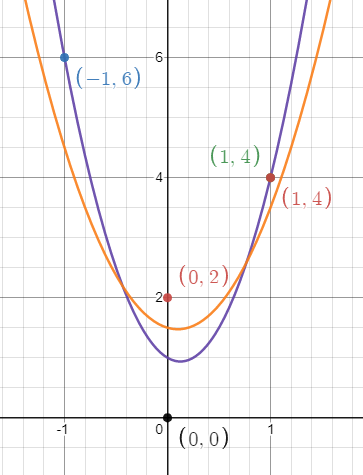
\includegraphics{task3.png}
\end{multicols}

\par 2)
\begin{align*}
& X = \begin{pmatrix}
    1 & 1 & 1 \\
    1 & 1 & 1 \\
    1 & 0 & 0 \\
    1 & 0 & 0 \\
    1 & -1 & -1
\end{pmatrix} \\
& y = \begin{pmatrix} 4 \\ 4 \\ 0 \\ 2 \\ 6 \end{pmatrix} \\
& X^T X = \begin{pmatrix}
    5 & 1 & 3 \\
    1 & 3 & 1 \\
    3 & 1 & 3
\end{pmatrix} \\
& X^T y = \begin{pmatrix} 16 \\ 2 \\ 14 \end{pmatrix} \\
& X^T X \beta = X^T y \\
& \begin{pmatrix}
    5 & 1 & 3 \\
    1 & 3 & 1 \\
    3 & 1 & 3
\end{pmatrix} \begin{pmatrix} \beta_1 \\ \beta_2 \\ \beta_3 \end{pmatrix} = \begin{pmatrix} 16 \\ 2 \\ 4 \end{pmatrix}
\Rightarrow \beta = \begin{pmatrix} 1 \\ -1 \\ 4 \end{pmatrix} \Rightarrow f(x) = 1 - x + 4x^2
\end{align*}

\par 3)
\begin{align*}
& \lambda = 1 \\
& X^T X + \lambda I = \begin{pmatrix}
    5 & 1 & 3 \\
    1 & 3 & 1 \\
    3 & 1 & 3
\end{pmatrix} + \begin{pmatrix}
    1 & 0 & 0 \\
    0 & 1 & 0 \\
    0 & 0 & 1
\end{pmatrix} = \begin{pmatrix}
    6 & 1 & 3 \\
    1 & 4 & 1 \\
    3 & 1 & 4
\end{pmatrix} \\
& (X^T X + \lambda I) \beta = X^T y \\
& \begin{pmatrix}
    6 & 1 & 3 \\
    1 & 4 & 1 \\
    3 & 1 & 4
\end{pmatrix} \begin{pmatrix} \beta_1 \\ \beta_2 \\ \beta_3 \end{pmatrix} = \begin{pmatrix} 16 \\ 2 \\ 14 \end{pmatrix}
\Rightarrow \beta = \begin{pmatrix} 1.5 \\ -0.5 \\ 2.5 \end{pmatrix} \Rightarrow f(x) = 1.5 - 0.5x + 2.5x^2
\end{align*}

\end{document}
